%!TEX root = ./template-skripsi.tex
%-------------------------------------------------------------------------------
%                            BAB III
%               			PEMBAHASAN
%-------------------------------------------------------------------------------

\chapter{METODOLOGI PENELITIAN}

\section{Keterhubungan Penelitian}

\begin{figure}[H]
	\centering
	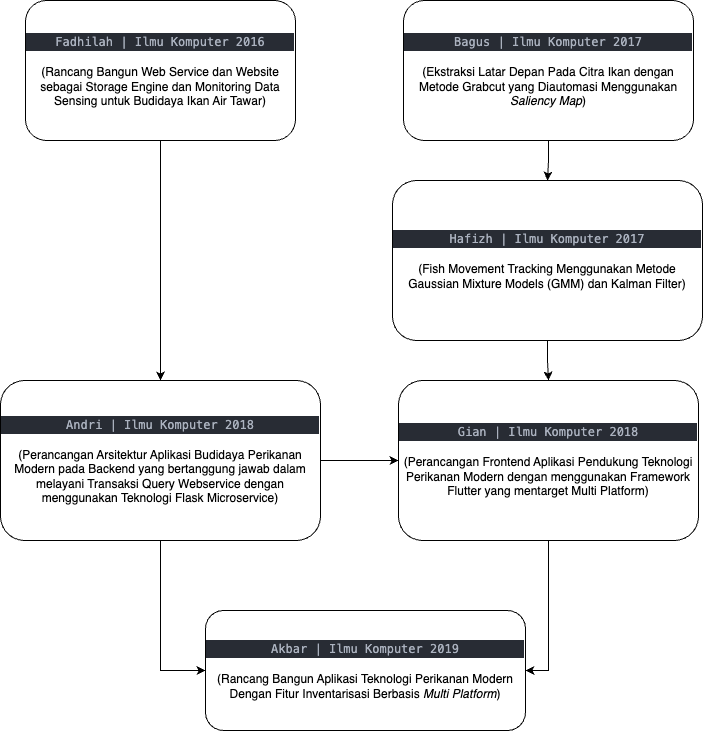
\includegraphics[width=0.7\textwidth]{gambar/akbar/research_tree.png}
	\caption{Diagram Alur Penelitian \textit{Aquaculture}}
\end{figure}

Pada diagram diatas, dapat dilihat urutan arah dari topik penelitian Aquaculture. Penelitian pertama kali dimulai oleh \citep{fadhil2021} dengan mengembangkan sebuah web service serta website yang berfungsi sebagai Storage Engine dan Monitoring Data Sensing untuk digunakan pada Budidaya Perikanan Air Tawar sebagai media penyimpanan data-data sensing dari sensor yang dikirimkan ke sistem serta memonitoringnya dalam bentuk table dan grafik real-time serta penelitian yang dilakukan oleh \citep{bagus2022} dengan tujuan untuk membangun sistem deteksi objek pada citra ikan dengan metode GrabCut yang telah diautomasi menggunakan \textit{saliency map}. 

Penelitian \citep{bagus2022} kemudian dilanjutkan oleh \citep{hafiz2021} yaitu merancang dan membangun sebuah sistem yang dapat melakukan pelacakan pergerakan ikan dengan menggunakan metode GMM dan Kalman Filter. Sementara penelitian \citep{fadhil2021} belum diterapkan pada aplikasi riset Aquaculture dalam waktu dekat sehingga penelitian yang dibuat oleh \citep{andri2022} dilakukan dengan membuat web service juga yang bertujuan untuk melayani transaksi query berupa monitoring budidaya perikanan yang dibarengi dengan penelitian \citep{gian2022} pada bagian perancangan \textit{frontend} sebagai pendukung pada aplikasi yang dikembangkan.

Dalam penelitian yang sudah berjalan ini, penulis mengembangkan penelitian yang dilakukan oleh \citep{andri2022} dan \citep{gian2022} dengan membuat fitur baru yaitu manajemen inventaris serta penentuan harga jual ikan dan penentuan upah pembudidaya ikan.

\section{Metode Penentuan Nilai Jual}

Dalam beberapa skenario, harga jual ditentukan oleh pedagang kepada pembudidaya. Harga ini dijamin lebih kecil dibanding harga retail, karena pedagang akan mengambil keuntungan dari itu. Jika dimisalkan T adalah harga jual minimum agar pembudidaya tidak rugi, $W_{feed}$ sebagai total pakan yang diberikan dan P adalah harga satuan pakan. Maka hubungan dari variabel-variabel tersebut adalah sebagai berikut.
\begin{equation}
    \begin{split}
		T
		&= W_{feed} \times P
    \end{split}
\end{equation}

Rumus ini didasari oleh konversi antara kilogram pakan menjadi pertambahan berat sebagian besar bervariasi tergantung pada kasus tertentu. Terlepas dari itu ditentukan oleh semakin tinggi asupan protein, maka semakin rendah tingkat konversinya. Jika konversi ini dikaitkan sebagai Food Conversion Ratio  (FCR) yang dimana $W_{fish}$ sebagai total berat dari semua ikan yang dipanen.
\begin{equation}
    \begin{split}
		FCR
		&= W_{feed } \div W_{fish}
    \end{split}
\end{equation}

Oleh karena itu, pembudidaya harus mencatat berapa banyak kilogram pakan yang diberikan sampai musim panen dari tiap kolam untuk menemukan nilai FCR-nya. Dalam masalah yang lebih kompleks, jika pakan memungkinkan datang dari berbagai sumber yang berhubungan dengan variasi asupan protein, FCR tidak dapat digunakan untuk menentukan hubungan antara jumlah pakan dan pertambahan berat.  Maka dari itu, sangat direkomendasikan untuk pembudidaya agar menggunakan satu sumber asupan protein tiap musim panen. Karena FCR sudah diketahui, selama musim panen berikutnya pembudidaya bisa memperkirakan berapa banyak pakan yang dibutuhkan untuk membuat ikan agar tumbuh sampai ukuran yang ditargetkan.
\begin{equation}
    \begin{split}
		W_{fish}
		&= W_{feed} \div FCR
    \end{split}
\end{equation}

Dengan itu bisa digunakan dalam mencari total jumlah pakan yang dibutuhkan untuk membuat ikan agar tumbuh sampai ukuran yang ditargetkan. 
\begin{equation}
    \begin{split}
		W_{feed}
		&= W_{fish} \times FCR
    \end{split}
\end{equation}

Jika persamaan 4 dikembangkan dengan memasukkan dua variabel yaitu $W_i$ sebagai berat ikan dan n sebagai jumlah ikan, maka persamaan akan menjadi seperti berikut.
\begin{equation}
    \begin{split}
		W_{fish}
		&= \sum_{i=1}^n \times W_i
    \end{split}
\end{equation}

Namun, menggunakan persamaan 5 akan mematikan tujuan dari persamaan 4, karena jika ingin menghitung pemakaian pakan diharuskan untuk menilai masing-masing ikan secara individu yang dimana itu tidak praktis. Jika menggunakan variabel $W_{af}$ sebagai rata-rata dari berat ikan, maka persamaan akan menjadi sebagai berikut.
\begin{equation}
    \begin{split}
		W_{af}
		&= \frac{\sum_{i=1}^n \times W_i}{n}
    \end{split}
\end{equation}

Sekarang dapat dengan mudah mencari perkiraan konsumsi pakan untuk musim panen berikutnya dengan persamaan,
\begin{equation}
    \begin{split}
		W_{feed}
		&= W_{af} \times n \times FCR
    \end{split}
\end{equation}


Jika persamaan 1 diupdate sehingga dapat ditemukan harga sesuai dengan persamaan,
\begin{equation}
    \begin{split}
		T_{unit}
		&= \frac{T}{n}
    \end{split}
\end{equation}

Persamaan itu juga merujuk pada jumlah perdagangan dalam kilogram, oleh karena itu
\begin{equation}
    \begin{split}
		k
		&= \frac{1kg}{W_{af}}
    \end{split}
\end{equation}

\begin{equation}
    \begin{split}
		T_k
		&= T_{unit} \times k
    \end{split}
\end{equation}

Sebagai contoh, dimisalkan mata uang yang digunakan adalah koin lalu FCR bernilai 1.5, ukuran target panen adalah 4 ikan per kilogram, di kolam terdapat 1000 ikan, dan harga pakan mencapai 10 koin.

Dari data tersebut, dapat diketahui $W_{af}$ = 1/4 kg, n = 1000. Karena itu, $W_{feed}$ bernilai 375 kg yang harus dipersiapkan. Selanjutnya, pembudidaya tidak bisa menjual semua hasil panen ikan seharga dibawah T = 3750 koin atau dibawah 15 koin per kilogram.

Persamaan 1 sampai 10 memungkinan jika FCR konstan dengan treatment yang sama dan asupan protein yang sama. Seperti yang sudah dilakukan diawal, pembudidaya harus mengandalkan satu sumber protein tetapi untuk mempertahankan hal ini sulit dilakukan. Karena itu, PER (Protein Efficiency Ratio) diketahui untuk menentukan rasio massa tubuh yang diperoleh dengan gram protein yang dikonsumsi. Disini variabel $P_{feed}$ mendefinisikan asupan gram protein.
\begin{equation}
    \begin{split}
		PER
		&= \frac{W_{fish}}{P_{feed}}
    \end{split}
\end{equation}

Pada formula tersebut, menggantikan $W_{feed}$ pada persamaan 2 dengan $P_{feed}$ akan memberikan bentuk variabel yang sama namun struktur variabel yang terbalik. Hal ini juga memberikan kemungkinan untuk mencampur beberapa sumber protein yang berbeda dengan formula berikut.
\begin{equation}
    \begin{split}
		PER
		&= \frac{W_{fish}}{P^1_{feed} + P^2_{feed} + \dots + P^k_{feed}}
    \end{split}
\end{equation}

\begin{equation}
    \begin{split}
		PER
		&= \frac{W_{fish}}{\sum_{i=1}^k \times P^i_{feed}}
    \end{split}
\end{equation}

Variabel k mengartikan jumlah dari sumber protein yang berbeda. Hal ini juga dapat dilakukan pada FCR dan T sebagai berikut.
\begin{equation}
    \begin{split}
		FCR
		&= \frac{\sum_{i=1}^k \times W^k_{feed}}{W_{fish}}
    \end{split}
\end{equation}
\begin{equation}
    \begin{split}
		T
		&= \sum_{i=1}^k \times W^k_{feed} \times P
    \end{split}
\end{equation}

Pada persamaan 15, hanya memodelkan harga jual minimum barang perikanan agar terhindar dari kerugian. Karena itu, untuk mendapatkan keuntungan diperlukan model yang baru. Disini variabel $T_p$ melambangkan dagangan yang memberikan keuntungan dan $F_g$ sebagai pendapatan pembudidaya.
\begin{equation}
    \begin{split}
		T_p
		&= T + F_g
    \end{split}
\end{equation}

$F_g$ merepresentasikan berapa banyak jam kerja yang dilakukan pembudidaya untuk membudidayakan ikan. Hal ini dapat dijelaskan lebih rinci dalam
\begin{equation}
    \begin{split}
		F_g
		&= D \times S
    \end{split}
\end{equation}

Dimana D mengartikan berapa banyak hari pembudidaya bekerja sampai musim panen dan S mengartikan upah yang mewakili pendapatan pekerjaan. Dalam berbudidaya, merupakan hal umum bagi pembudidaya ikan untuk menghabiskan waktu seharian penuh untuk mengembangkan dan memantau kolam, karena itu representasi hari lebih ideal. Sebab itu, pembudidaya yang lebih banyak menghabiskan waktunya sampai musim panen tiba harus mendapatkan pendapatan yang sesuai.

Persamaan 15 berlaku jika budidaya ikan membudidayakan ikan tradisional secara tradisional. Dalam sistem intensif aquaculture khususnya BFT, dibutuhkan variabel yang mewakili biaya tambahan yang dikeluarkan untuk penggunaan teknologi. Variabel ${C_i}$ merepresentasikan masing-masing biaya tambahan yang dikeluarkan dalam BFT untuk keseluruhan musim kawin.
\begin{equation}
    \begin{split}
		T
		&= \sum_{i=1}^k \times W^k_{feed} \times P + \sum_{i=1}^l \times C_i
    \end{split}
\end{equation}

Variabel $C_i$ dapat dijabarkan sebagai berikut.

\begin{itemize}
	\item $C_1$ = Bahan Baku
	\item $C_2$ = Listrik (dihitung dalam per Kolam)
	\item $C_3$ = Tenaga Kerja (dihitung 3-5 jam / orang serta dibagi dengan jumlah kolam)
	\item $C_4$ = Benih Ikan
\end{itemize}

Dalam menyimpan bahan baku pada inventaris, bahan baku tersebut akan mengalami penurunan karena bahan baku mempunyai masa kadaluarsa. Seiring dengan lamanya bahan baku tersebut disimpan, tentunya semakin lama bahan baku tersebut akan menurun kualitasnnya sampai masa kadaluarsa dari bahan baku tersebut tercapai. Maka dari itu, dapat dimisalkan jika per bulan bahan baku tersebut mengalami penurunan kualitas sebesar 25\% dari harga belinya, maka dalam 4 bulan bahan baku tersebut akan kadaluarsa dan sudah tidak lagi berharga. Namun, skala penurunan tersebut bervariasi tergantung pada jenis bahan baku yang digunakan. Variabel $W_p$ mewakili harga dari bahan baku yang digunakan dan variabel $\alpha$ mewakili skala depresiasi per bulan dari bahan baku yang digunakan. Formula depresiasi dapat dibuat menjadi persamaan berikut.

\begin{equation}
    \begin{split}
		W_p
		&= W_p - \alpha \times W_p
    \end{split}
\end{equation}

\section{Analisa Arsitektur Fitur}

Pada penelitian aplikasi yang sudah dikembangkan sebelumnya, terdapat use case yang menjelaskan konsep dari aplikasi yang ada pada gambar dibawah ini.

\begin{figure}[H]
	\centering
	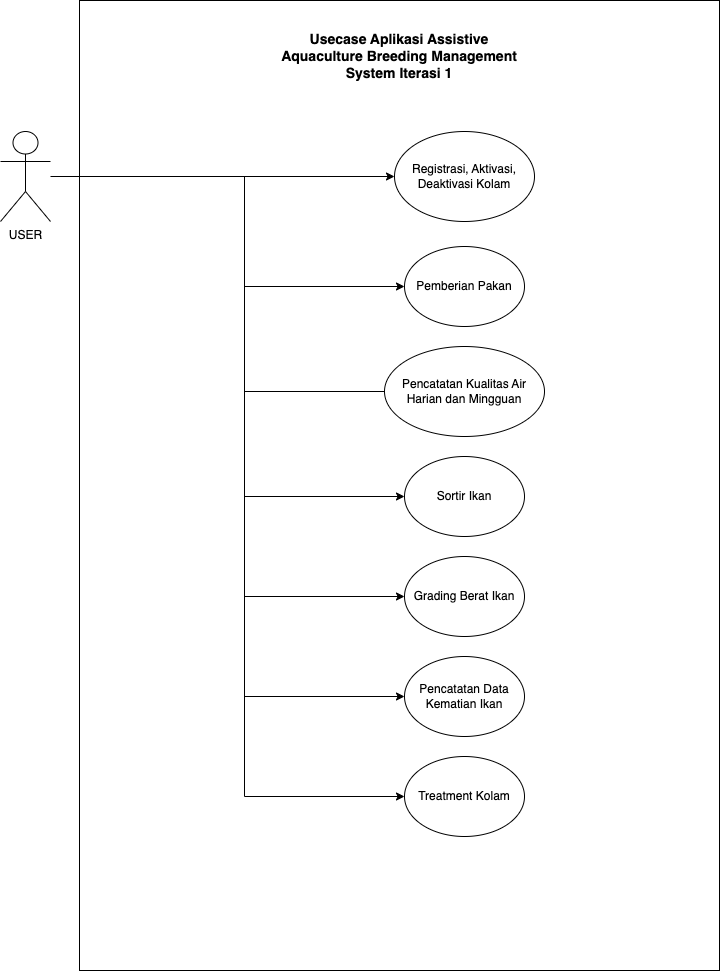
\includegraphics[width=0.7\textwidth]{gambar/akbar/usecase_iterasi_1.png}
	\caption{Use Case Fitur Aplikasi pada Iterasi 1}
\end{figure}

Dari diagram use case tersebut, terdapat dua jenis pengguna yaitu user dan admin. User dan admin memiliki fitur yang sama dalam aplikasi tersebut, yang membedakan antara user dan admin adalah skala prioritas dari aplikasi. Sisi admin memungkinkan pengguna dapat mengatur lebih banyak fitur yang ada pada aplikasi dan mendapatkan akses untuk mengatur user non-admin. Fitur yang disediakan aplikasi dijelaskan sebagai berikut.

\begin{enumerate}
	\item \textbf{Registrasi, Aktivasi, Deaktivasi Kolam} = Fitur ini digunakan untuk mendaftarkan kolam yang akan dijadikan tempat budidaya ikan, kemudian fitur aktivasi dan deaktivasi kolam digunakan untuk mengontrol kolam yang sedang berjalan.
	\item \textbf{Pemberian Pakan} = Fitur ini digunakan untuk mencatat data pakan yang diberikan pada kolam ikan di budidaya yang sedang berlangsung.
	\item \textbf{Pencatatan Kualitas Air Harian dan Mingguan} = Fitur ini digunakan untuk mencatat kualitas air dari kolam di budidaya yang sedang berjalan dengan rentang waktu harian dan mingguan.
	\item \textbf{Sortir Ikan} = Fitur ini digunakan untuk mengatur perpindahan ikan ke kolam lain.
	\item \textbf{Grading Berat Ikan} = Fitur ini digunakan untuk mengatur ekosistem ikan berdasarkan berat agar mendapatkan keseragaman ukuran ikan dan meningkatkan efektivitas pemberikan pakan kepada ikan.
	\item \textbf{Pencatatan Data Kematian Ikan} = Fitur ini digunakan untuk mencatat angka kematian ikan jika terdapat ikan yang mati ketika budidaya sedang berjalan.
	\item \textbf{Treatment Kolam} = Fitur ini digunakan untuk melakukan pengaturan terhadap kolam ikan pada budidaya yang sedang berjalan.
\end{enumerate}

\section{Analisa Pengembangan Fitur}

Dalam Iterasi 2 ini, fitur yang ditambahkan adalah fitur manajemen inventaris. Pada analisa arsitektur fitur yang ada di aplikasi sebelumnya, dapat dilengkapi dengan fitur inventaris yang akan dilakukan pada penelitian ini. Fitur tersebut memiliki use case diagram dengan referensi dari use case diagram aplikasi sebelumnya seperti berikut.

\begin{figure}[H]
	\centering
	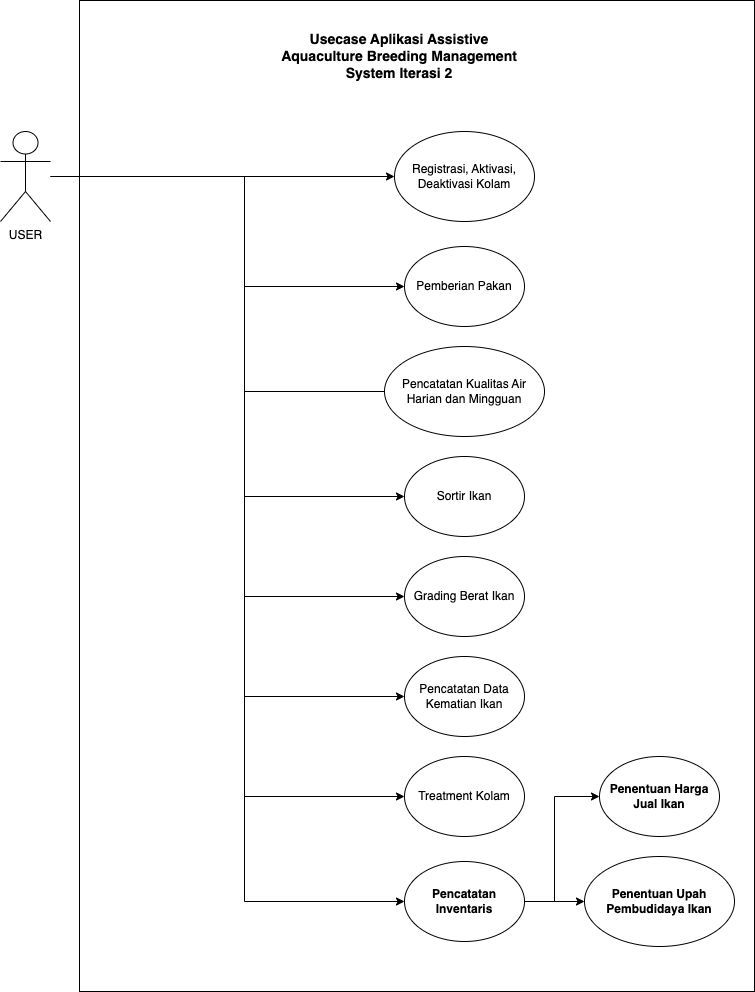
\includegraphics[width=0.7\textwidth]{gambar/akbar/usecase_iterasi_2.png}
	\caption{Use Case Fitur Aplikasi pada Iterasi 2}
\end{figure}

Fitur pencatatan inventaris merupakan fitur yang akan ada pada aplikasi yang berguna untuk para pembudidaya ikan mencatat semua hal yang berhubungan dengan budidaya perikanannya. Hal-hal yang dapat dicatat oleh pembudidaya pada fitur ini adalah sebagai berikut.

\begin{enumerate}
	\item Bahan Baku Pakan
	\item Bahan Baku Material Organik
	\item Listrik
	\item Benih Ikan
	\item Peralatan
\end{enumerate}

Selain mencatat inventaris pada budidaya, fitur pencatatan inventaris ini juga dapat menentukan harga jual dari ikan yang dipanen serta dapat juga menentukan upah layak dari pembudidaya ikan berdasarkan formula yang ada pada persamaan 3.18.

\section{Perancangan Sistem}

Dalam mengembangkan fitur yang ada pada Iterasi 2 ini, penelitian dilakukan dengan metode Scrum. Metode Scrum merupakan metode yang sering digunakan dalam develop sebuah aplikasi karena dapat menyelesaikan masalah kompleks dengan efektif. Berikut penjelasan dari masing-masing elemen yang ada pada metode Scrum.

\subsection{Product Backlog}

Product Backlog adalah tugas-tugas yang \textbf{akan} dijalankan pada penelitian dan hal yang pertama kali dilakukan sebelum memulai riset. Daftar tugas yang ada pada Product Backlog ini akan dipindahkan pada Sprint Backlog tergantung pada skala prioritas dari task itu sendiiri. Berikut adalah tabel dari Product Backlog yang sudah berjalan.

\begin{table}[H]	
	\begin{center}
		\caption{Tabel Product Backlog}
		\label{tab:table5}
		\begin{tabular}{|c|m{17em}|c|c|}
		\hline
		\textbf{No} & \textbf{Stories} & \textbf{Sprint} & \textbf{Status} \\
		\hline
		1 & Membuat fitur pencatatan inventaris & 1 & On Progress \\
		\hline
		2 & Membuat fitur depresiasi aset dalam inventaris & - & Uncomplete \\
		\hline
		3 & Membuat fitur penentuan nilai jual ikan & - & Uncomplete \\
		\hline
		4 & Membuat fitur sortir yang terkoneksi dengan harga & - & Uncomplete \\
		\hline
		5 & Membuat fitur pemberian pakan yang terkoneksi dengan inventaris & - & Uncomplete \\
		\hline
		6 & Membuat fitur panen yang terhitung dengan harga riil & - & Uncomplete \\
		\hline
		7 & Membuat fitur pemetaan sebaran ikan terpanen & - & Uncomplete \\
		\hline
		8 & Membuat fitur penentuan upah kerja pembudidaya & - & Uncomplete \\
		\hline
		\end{tabular}
	\end{center}
\end{table}

\subsection{Sprint Backlog}

Sprint Backlog adalah daftar tugas yang \textbf{harus} dijalankan selama masa Sprint berlangsung. Tugas yang ada pada Sprint Backlog bersifat fleksibel seiring dengan berjalannya Sprint. Berikut merupakan tabel dari Sprint Backlog yang sudah berjalan.

\begin{table}[H]	
	\begin{center}
		\caption{Tabel Sprint 1 Backlog}
		\label{tab:table6}
		\begin{tabular}{|c|c|m{13em}|c|}
		\hline
		\textbf{No} & \textbf{Stories} & \textbf{Task} & \textbf{Status} \\
		\hline
		% 1 & Membuat fitur pencatatan inventaris & Membuat skema database dari pencatatan inventaris & User & 1 & Uncomplete \\
		%  &  & Membuat mockup dari fitur inventaris & User & 1 & Uncomplete \\
		1 & \multirow{2}{10em}{Membuat fitur pencatatan inventaris} & - Membuat skema database dari pencatatan inventaris & On Progress \\
		&  & - Membuat mockup dari fitur inventaris & On Progress \\ 
		\hline
		\end{tabular}
	\end{center}
\end{table}

\subsection{Sprint}

Sprint merupakan kegiatan menyelesaikan daftar tugas yang ada pada Sprint Backlog dalam rentang waktu tertentu. Durasi Sprint sendiri bermacam-macam, bisa dari 1-4 minggu tergantung dari kesulitan tugas itu sendiri. Berikut merupakan list Sprint yang sudah berjalan.

\begin{enumerate}
	\item Sprint 1
	
	Sprint 1 dilaksanakan pada tanggal 15 Februari 2023 - XX Maret 2023. Pada sprint ini mengerjakan tugas yang ada pada Sprint 1 Backlog di Tabel 3.2.
\end{enumerate}

\subsection{Daily Scrum}

Daily Scrum merupakan kegiatan rutin tiap minggu yang dilaksanakan dengan Scrum Master. Kegiatan ini dilakukan untuk reporting progres tugas yang dijalankan selama masa Sprint berlangsung kepada Scrum Master. Scrum Master bertugas untuk memberikan feedback saat Daily Scrum berlangsung.

\subsection{Sprint Review dan Sprint Restropective}

Sprint Review dan Sprint Restropective adalah kegiatan mengulas kembali tugas yang sudah dikerjakan pada saat durasi Sprint berlangsung. Kegiatan ini juga merupakan kegiatan menentukan tugas yang berhasil dan tidak berhasil selama Sprint berlangsung.

\subsection{Sprint 1 Report}

Tujuan dari Sprint 1 ini adalah membuat skema database dari inventarisasi serta membuat mockup design dari fitur inventaris yang akan diterapkan pada aplikasi.

\begin{enumerate}
	\item Membuat skema database inventaris
	
	Berikut merupakan skema database yang mewakili fitur inventaris dapat dilihat pada Gambar 3.4 berikut.

	\begin{figure}[H]
		\centering
		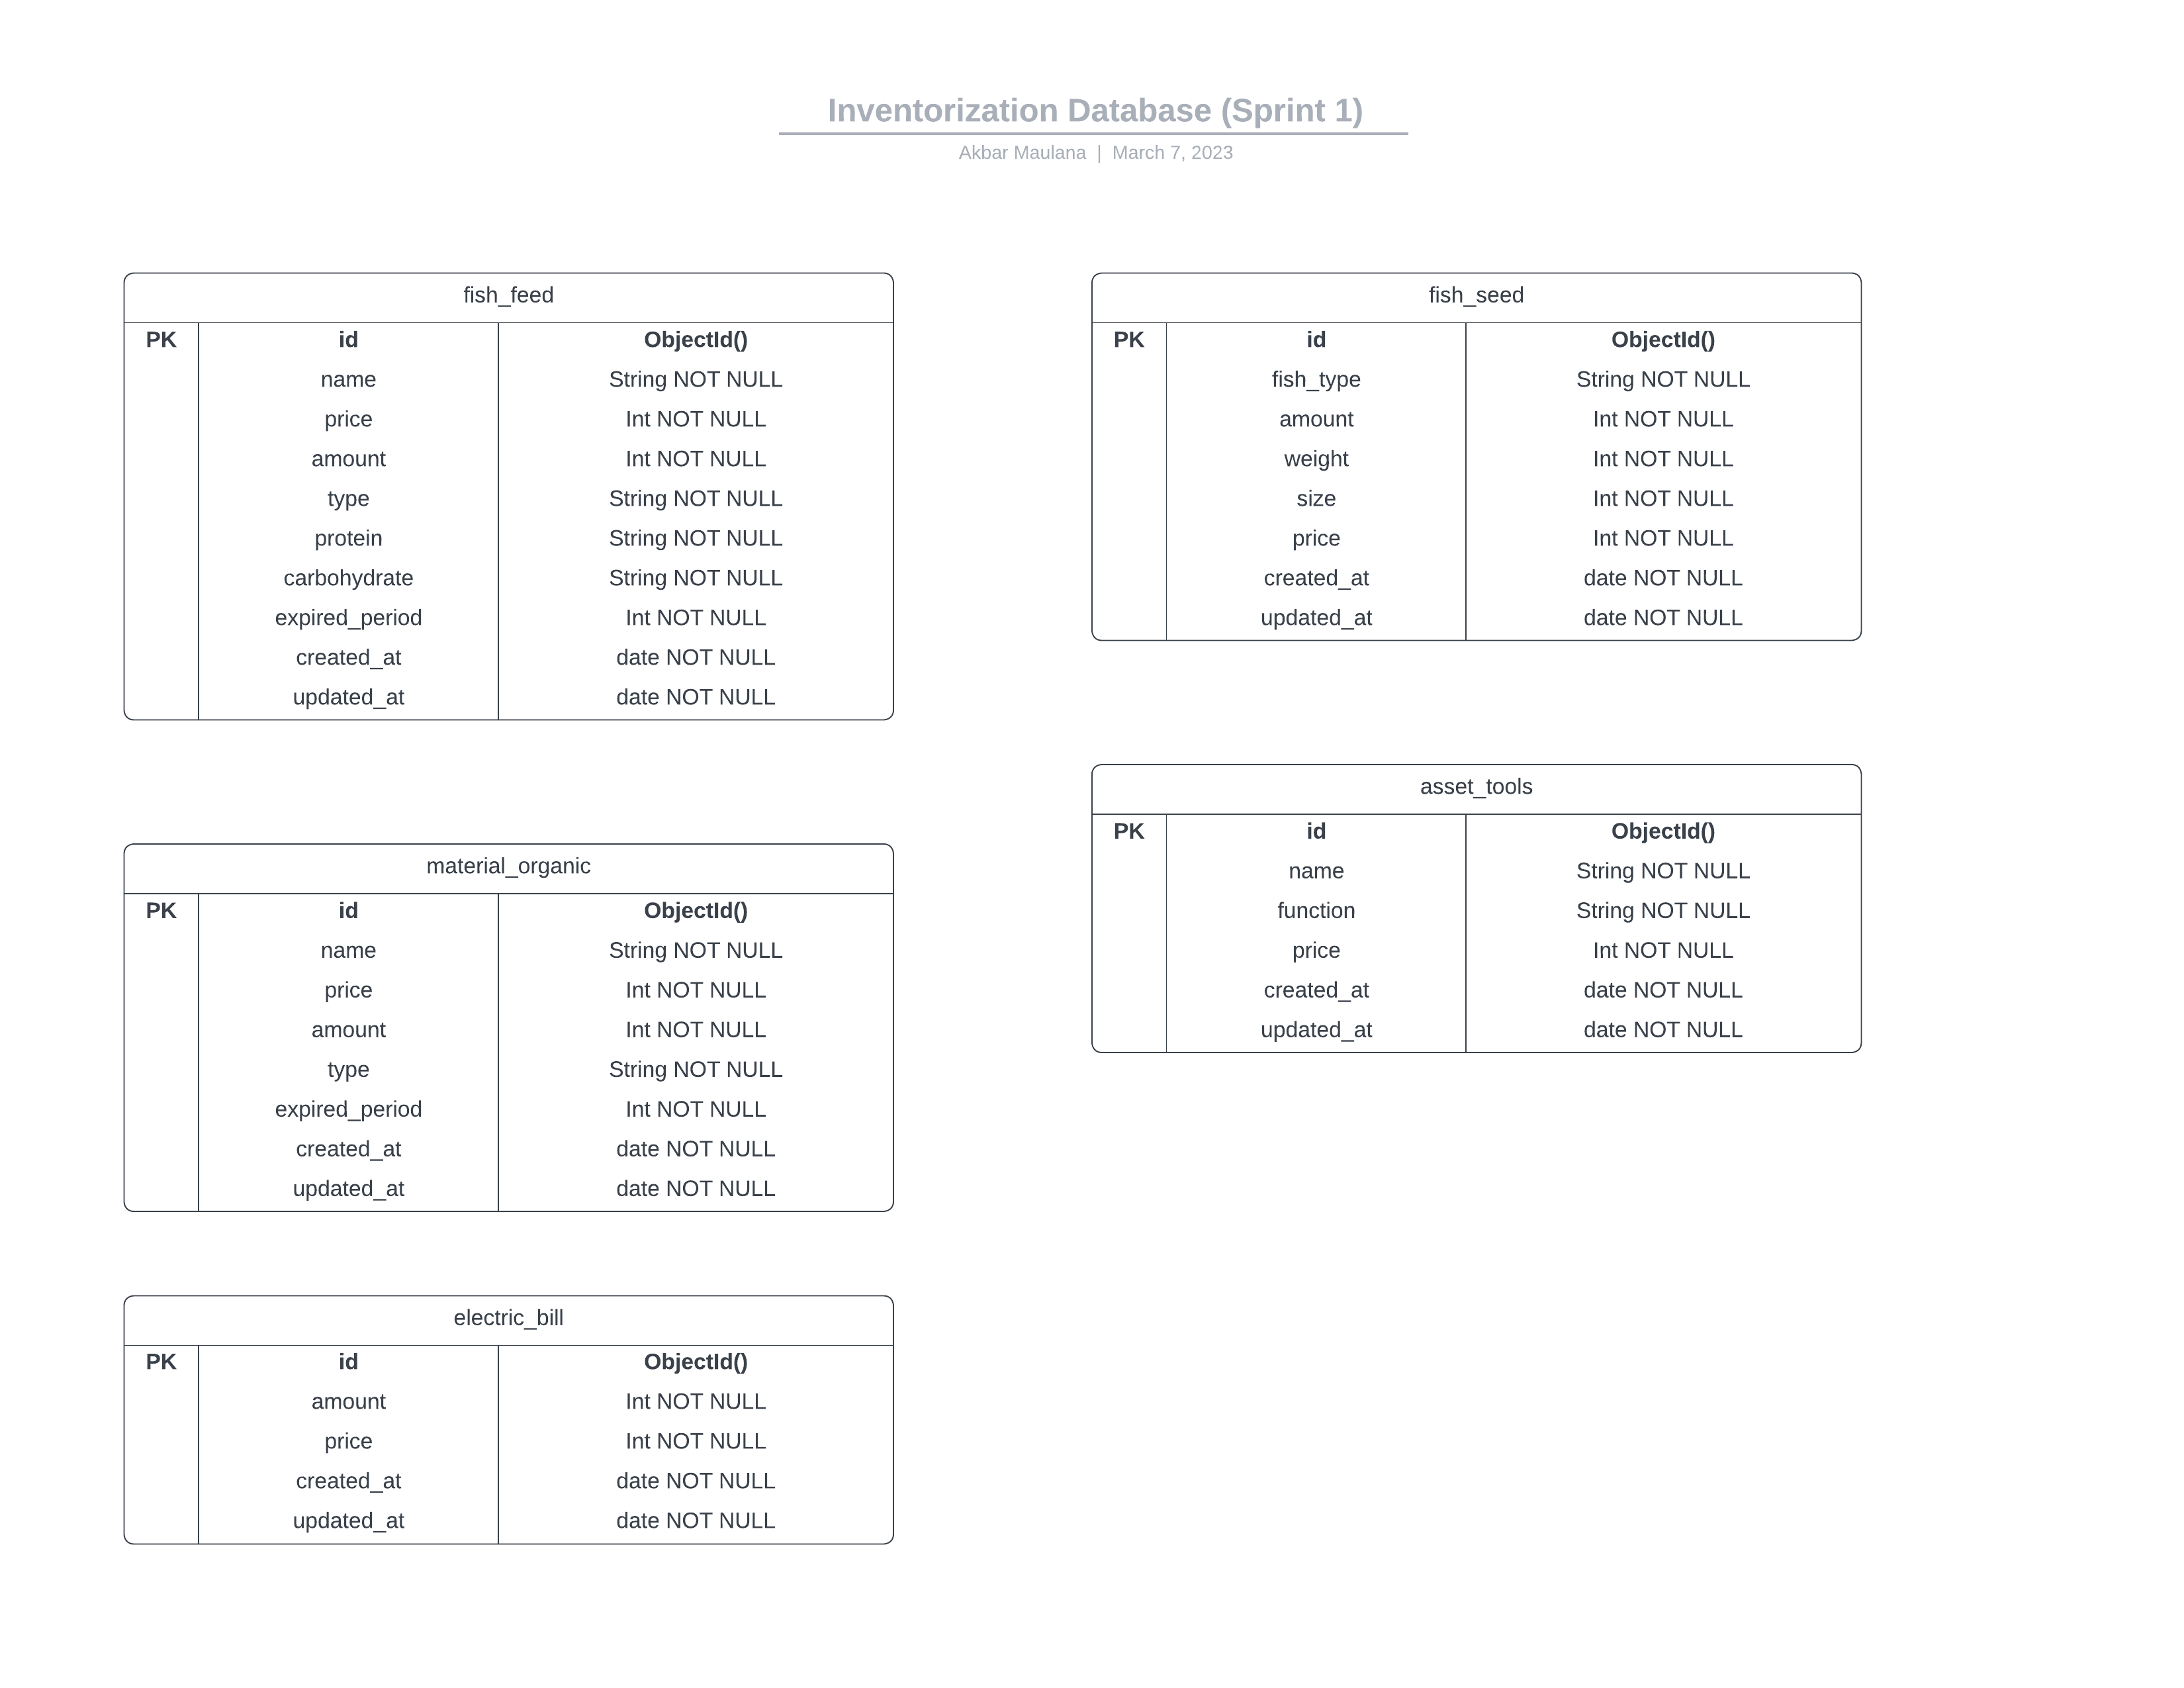
\includegraphics[width=1\textwidth]{gambar/akbar/sprint1/sprint1_inventaris_database.png}
		\caption{Skema Database Fitur Inventaris}
	\end{figure}

	Dari skema database tersebut, terdapat lima opsi kategori inventaris yang sudah dijelaskan sebelumnya. Pada skema database ini, masing-masing kategori memiliki kebutuhan yang berbeda antara lain.

	\begin{enumerate}
		\item fish\_feed (Pakan Ikan)
		\item material\_organic (Bahan Organik)
		\item electric\_bill (Tagihan Listrik)
		\item fish\_seed (Benih Ikan)
		\item asset\_tools (Peralatan)
	\end{enumerate}

	Dalam tabel database tersebut, pada kolom pertama terdapat jenis \textit{key} yang dijadikan patokan dalam tabel database tersebut. Kemudian kolom kedua dan ketiga merupakan hubungan antara nama data dan tipe data yang mewakili nama data tersebut.

	Setelah skema database dari inventaris telah dibuat, tabel-tabel database tersebut harus diintegrasikan dengan skema database sebelumnya untuk menyesuaikan kebutuhan fitur yang akan dibuat nantinya. Berikut merupakan skema database yang telah diintegrasikan dengan skema database dari inventaris dapat dilihat pada Gambar 3.5.

	\begin{figure}[H]
		\centering
		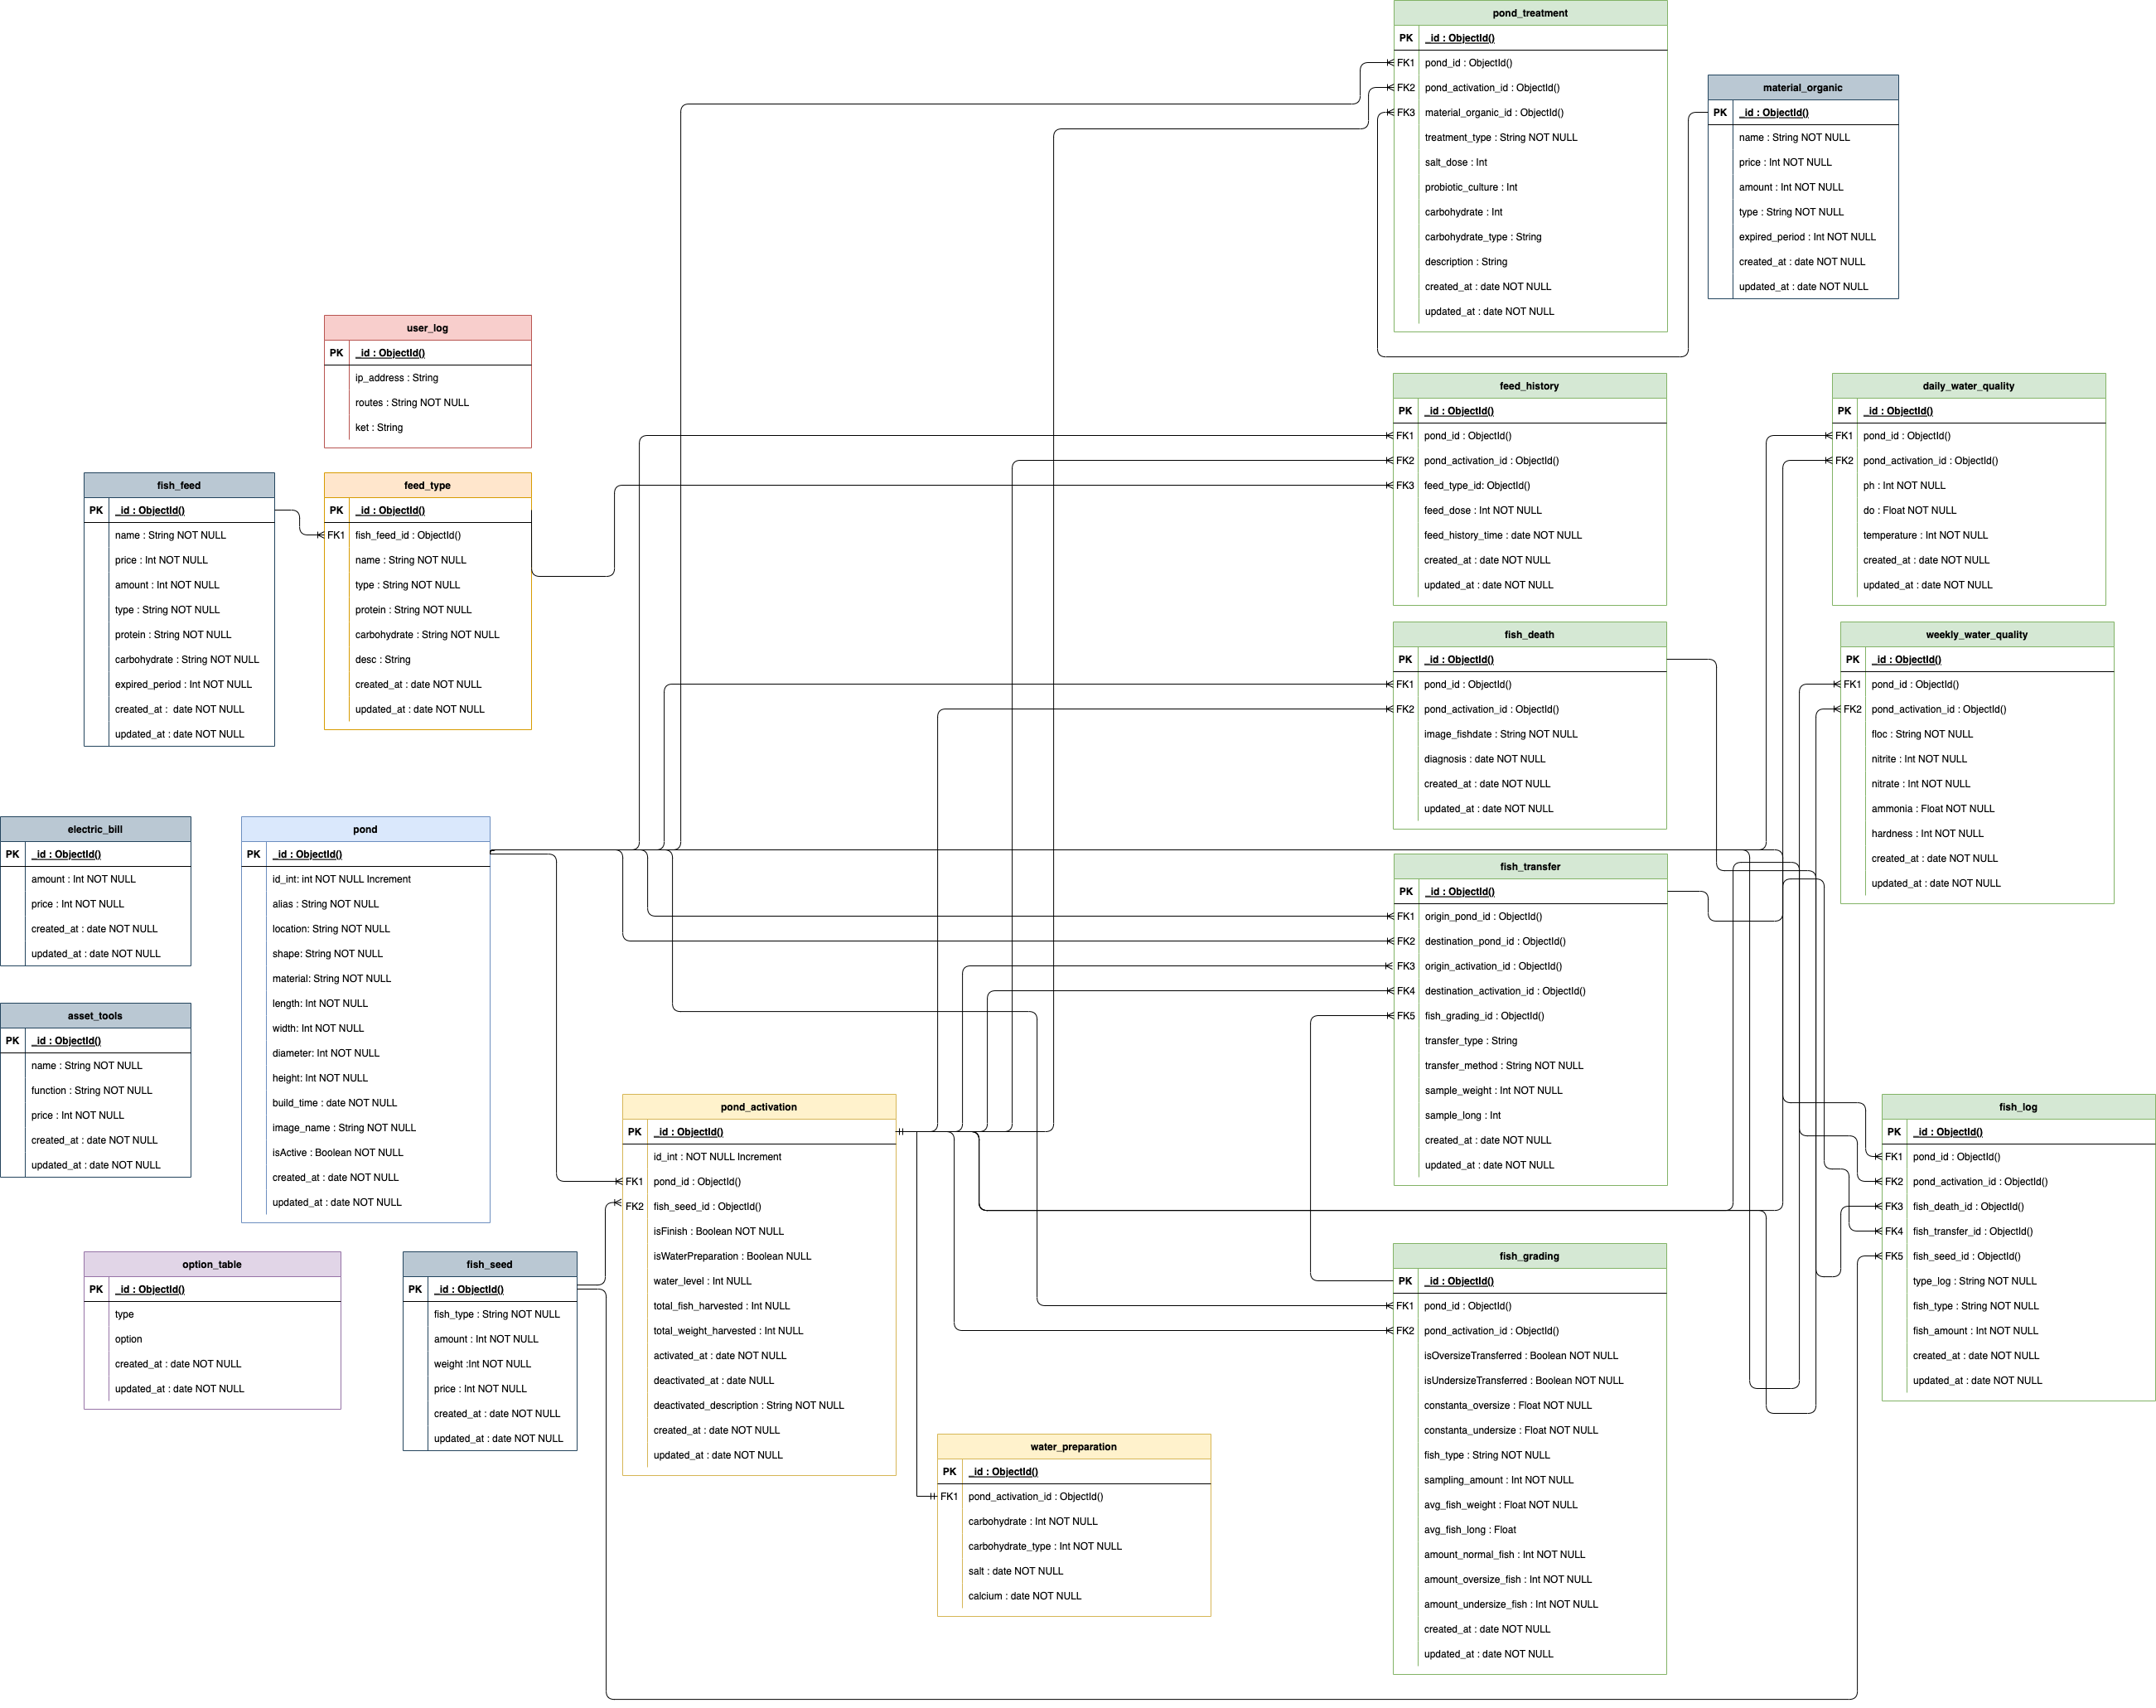
\includegraphics[width=1\textwidth]{gambar/akbar/sprint1/sprint1_skema_database.png}
		\caption{Integrasi Skema Database Inventaris dengan Skema Database Iterasi 1}
	\end{figure}

	\item Membuat mockup design halaman inventaris
	
	Dalam membuat mockup design ini, 

	Berikut merupakan mockup dari fitur inventaris berdasarkan skema database yang sudah dibuat sebelumnya.
\end{enumerate}